
\chapter{Introduction}

\section{Overview}

The Federal Highway Administration (FHWA) conducts research in an effort to improve road safety. The FHWA is interested in where car accidents happen on a given road. Knowing the location of accidents on a road can help the FHWA determine which segments of a road are dangerous. The purpose of this project is to model car crashes on segments of a road based on variables such as road characteristics (type of pavement, shoulder width, number of lanes, etc.) and annual average daily traffic. By doing this, we hope to be able to identify segments of road that have more accidents than they should.  Using the results of this model, the FHWA identify and make changes to those dangerous road segments to make roads safer and reduce the number of crashes.

\section{Data}

The Highway Safety Information System (HSIS) is a roadway-based system that provides data about crash, roadway, and traffic variables. HSIS is currently managed by the University of North Carolina Highway Safety Research Center (HSRC) under contract with FHWA. Each state involved in the HSIS research project collects data independently of HSIS-- the data from each state is gathered by HSIS on an annual basis. Data can be requested from the HSIS for analysis. For each state, HSIS has up to seven different data files: crash, roadway, traffic volume, curve/grade, intersection, and interchange. For the purpose of this analysis, only the crash and roadlog files were used. The crash data files for each state are split up into two seperate files: a crash file, and a vehicle file. The crash file contains information on each crash while the vehicle file contains information on each vehicle and each driver of each crash. The roadlog file contains information on homogeneous sections of roads such as number of lanes, lane width, annual average daily traffic, etc.


There are currently nine states in the HSIS data base. These nine states were selected primarily because of the availability of data; meaning the data that these states collect contain all the variables of interest as well as a high quantity and quality of information gathered. The selected states are: California, Illinoise, Maine, Minnesota, Michigan, Ohio, North Carolina, Utah, and Washington. However, HSIS stopped recieving data from Utah and Michigan in 2000 and 1997 because of changes in inventory data collection.

For the purpose of my thesis, I will be focusing on road segments in Minnesota. The data used come from 2011 and 2012.  The following table contains all covariates that will be used as a part of the analysis. 

% \usepackage{booktabs}
\begin{table}[h]
\centering
\caption{Minnesota covariates}
\label{my-label}
\begin{tabular}{@{}ll@{}}
\toprule
aadt      & Average annual daily traffic         \\ 
medwid    & Median width (feet)                  \\
med\_type & Median type                          \\
lshldwid  & Left shoulder width - road 1 (feet)  \\
surf\_wid & Surface width - road 1 (feet)        \\
rshldwid  & Right shoulder width - road 1 (feet) \\
rshl\_typ & Right shoulder type - road 1         \\
func\_cls & Functional class                     \\
no\_lanes & Total number of lanes                \\
lanewid   & Lane width                           \\
rodwycls  & Roadway classification               \\ \bottomrule
\end{tabular}
\end{table}

Below are graphs of crashes along the Interstate 35 and Interstate 94. The expected number of crashes was calculated using annual average daily traffic on each road segment. The expected number of crashes for segment s is: $E_s = \frac{\sum_s Y_s}{\sum_s AADT_s * length_s} * AADT_s * length_s$

\centerline{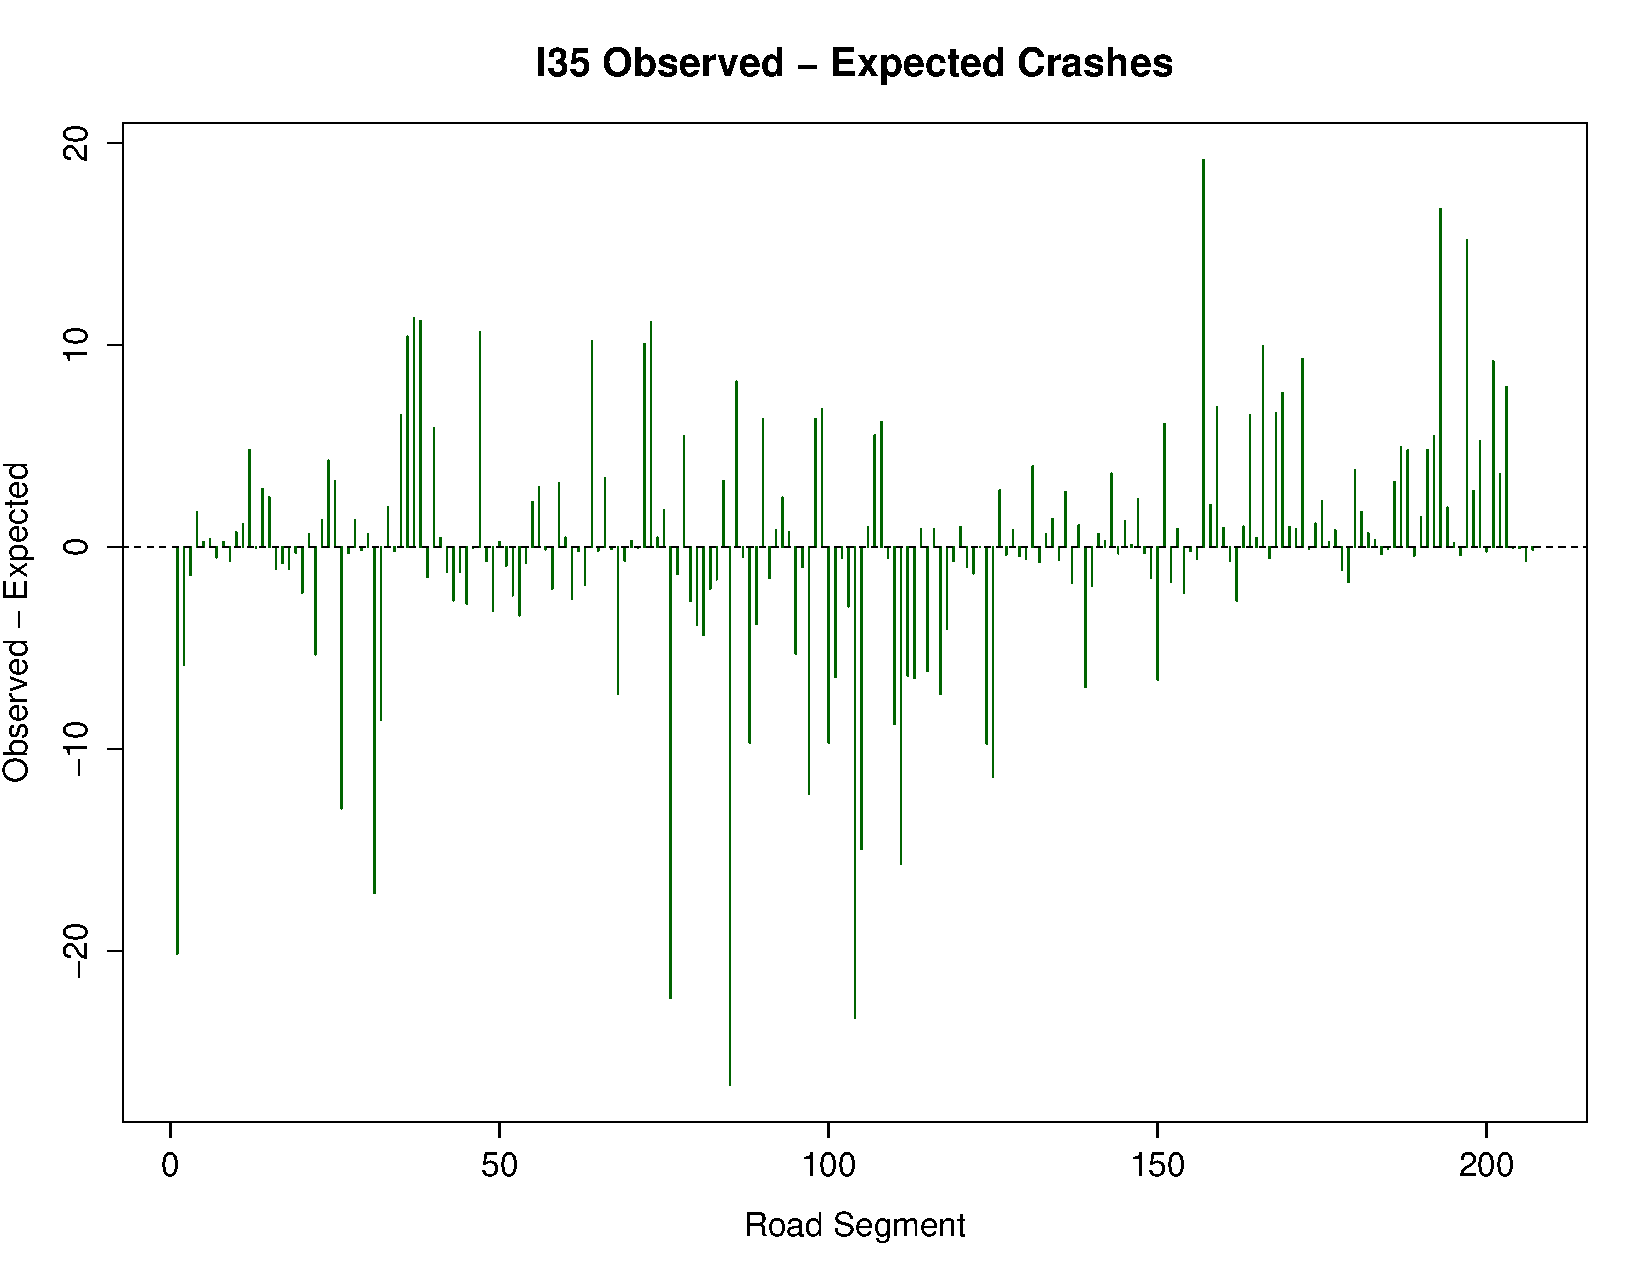
\includegraphics[width=.9\textwidth]{i35crash.pdf}}
\centerline{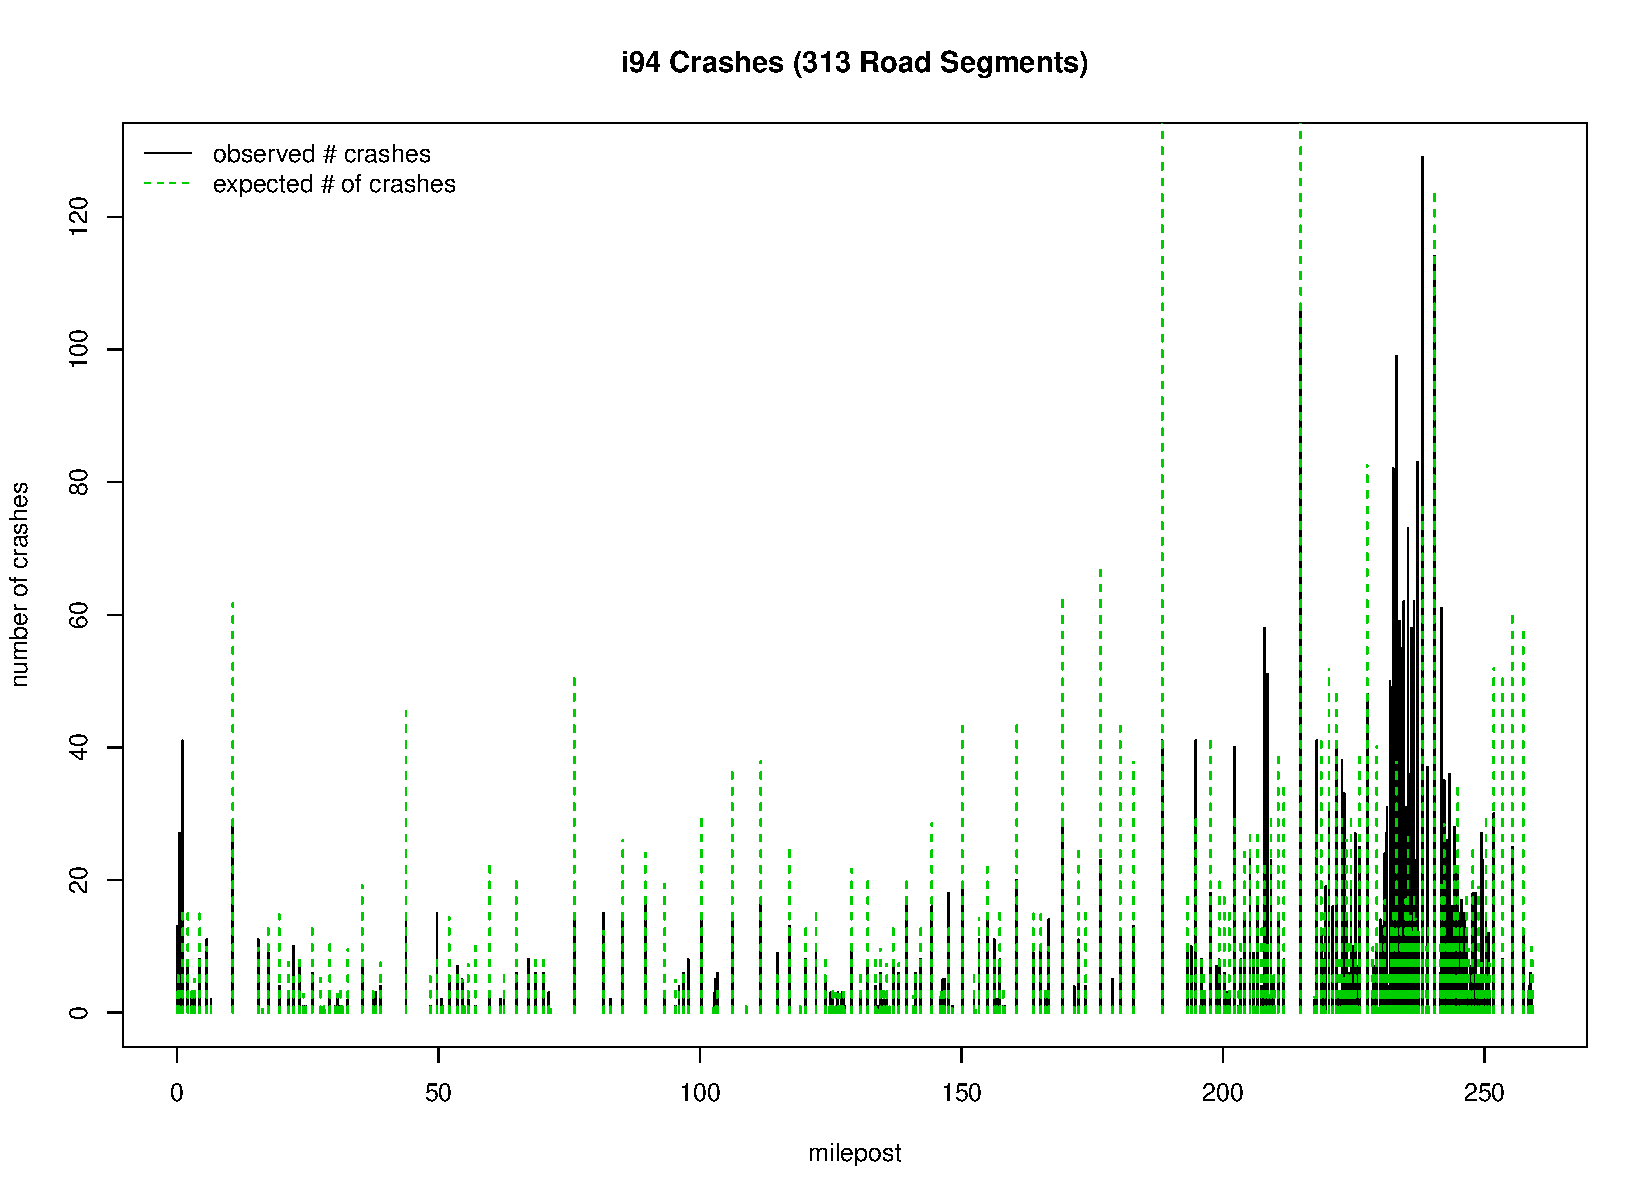
\includegraphics[width=.9\textwidth]{i94crash.pdf}}


\section{Modeling Challenges}

\textbf{Spatial Correlation:} Spatial correlation is the idea that locations that are close (in time or space) together tend to have similar characteristics. In the case of this project, segments of road that are connected will most likely have a high correlation because of their closeness in space. This can be seen in the graphs on page x. Look at figure 2 (I94 crashes). From milepost 0 to 200 number of crashes are relatively stable and low, but from milepost 200 to 250, the number of crashes (as well as the variabilty) drastically increases. If there were no spatial correlation, then those spikes found from mile post 200 to 250 would have been more evenly distributed throughout the data.

%\noindent
%\textbf{Computational Challenges:}

\noindent
\textbf{Linear Regression:} Since we are modeling count data, standard linear regression techiniques will not work. Linear regression would produce a model that could potentially predict negative and/or non-integer number of crashes. 

\noindent
\textbf{Autocorrelation:} Inherent in the data is some measure of autocorrelation. For instance, average annual daily traffic and the number of lanes are highly correlated as one would expect (a higher number of lanes typically indicates a greater volume of traffic flowing through a street).  Because of this, we will use a variable selection technique to trim down the number of covariates.

\section{Methods Overview}
%In this section you need to give an overview of your model (not too specific) and why it meets the challenges you stated above.
%\begin{enumerate}
%\item State that you are going to do a Poisson regression with spatially varying effects.
%\item Talk briefly (no specifics yet) about what a CAR model is and how it ties things together spatially.
%\item  State that you are going to use a Bayesian LASSO for variable selection/shrinkage.
%\end{enumerate}

We will model the data using a Poisson regression with spatially varying effects. A Poisson regression ensures that we are modeling count data (integers greater than zero) and by including spatially varying effects we will capture the spatial depency inherent in the data. To include spatial effects, we will use a conditional autoregressive (CAR) model. A CAR model is appropriate to fit the data because the data is areal (region specific as opposed to point specific locations). To correct for autocorrelation, we will use a Bayesian LASSO to shrink autocorrelated variables to zero. 
